% Number 471
% UFPM Normal
% Accel. elevator: v up, slowing down
% MIT

% Watermark
\AddToShipoutPicture*{\BackgroundPic}

\addtocounter {ProbNum} {1}

\begin{floatingfigure}[r]{.2\textwidth}
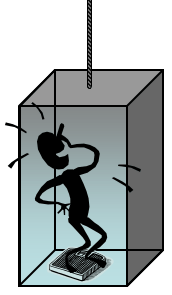
\includegraphics[scale=.6]{/Users/jgates/desktop/latex/pics/scaleinelevator1}
\end{floatingfigure}
 
{\bf \Large{\arabic{ProbNum}}} An elevator contains an 85 kg physicist standing on a scale. The elevator is moving upwards at a rate of ${2~\tfrac{m}{s}}$ and slowing down at a rate of ${3~\tfrac{m}{s^2}}$.

\bigskip
What does the scale read?


%\begin{center}
%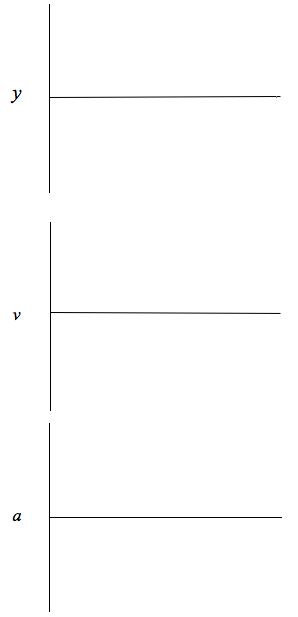
\includegraphics[scale=.85]{/Users/jgates/desktop/latex/pics/blankyvagraphstack.png}
%\end{center}


\vfill
\newpage
